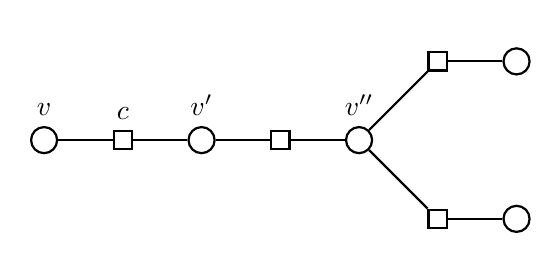
\begin{tikzpicture}[thick,scale=1]
\node[circle,draw=black,label={$v$}] (v1) at (-2,0){};
\node[circle,draw=black,label={$v'$}] (v2) at (0,0){};
\node[circle,draw=black,label={$v''$}] (v3) at (2,0){};
\node[circle,draw=black,label={}] (v4) at (4,1){};
%\node[circle,draw=black,label={}] (v5) at (-2,2){};
%\node[circle,draw=black,label={$v$}] (v6) at (2,2){};
%\node[circle,draw=black,label={}] (v7) at (2,-2){};
\node[circle,draw=black,label={}] (v8) at (4,-1){};

\node[shape=rectangle,draw=black,label={$c$}] (c1) at (-1,0){};
\node[shape=rectangle,draw=black,label={}] (c2) at (1,0){};
\node[shape=rectangle,draw=black,label={}] (c3) at (3,1){};
\node[shape=rectangle,draw=black,label={}] (c4) at (3,-1){};
%\node[shape=rectangle,draw=black,label={}] (c4) at (0,2){};
%\node[shape=rectangle,draw=black,label={}] (c5) at (4,-2){};



\path [-,thick] (v1) edge node[left] {} (c1); 
\path [-,thick] (v2) edge node[left] {} (c1);
\path [-,thick] (v2) edge node[left] {} (c2);
\path [-,thick] (v3) edge node[left] {} (c2);
\path [-,thick] (v4) edge node[left] {} (c3);
\path [-,thick] (v3) edge node[left] {} (c3);
%%%%%%%%
\path [-,thick] (v8) edge node[left] {} (c4);
\path [-,thick] (v3) edge node[left] {} (c4);
%%%%%%%%%%%%
%\path [-,thick] (v6) edge node[left] {} (c2);
%\path [-,thick] (v7) edge node[left] {} (c2);
%\path [-,thick] (v7) edge node[left] {} (c5);
%\path [-,thick] (v8) edge node[left] {} (c5);
\end{tikzpicture}